\section{Bài tập 2}
\subsection{Eager Beaver}
Điều kiện của $a$, $b$ trong phong cách này là $a>0$ và $b>0$. Ta xét 2 ví dụ cùng ma trận hệ số nhưng điều kiện ban đầu khác nhau.
\subsubsection{Ví dụ 1}
\begin{align*}
    \begin{cases}
        R'=R+2J\\
        J'=3R+2J\\
        R(0)=0\\
        J(0)=-4
    \end{cases}
\end{align*}
Theo bài 1, ta có $\Delta=25>0$, hệ có 2 trị riêng phân biệt $\lambda_1=-1, \lambda_2=4$. Áp dụng công thức nghiệm chính xác ở trường hợp 1:
\begin{align*}
    \begin{cases}
        R(t)=\frac{8}{5}e^{-t}-\frac{8}{5}e^{4t}\\
        J(t)=-\frac{8}{5}e^{-t}+-\frac{12}{5}e^{4t}
    \end{cases}
\end{align*}
Biểu diễn $R$ (eager beaver) và $J$ (eager beaver) trên cùng một đồ thị theo biến thời gian $t$ (hình 1):
\begin{figure}[h!]
    \begin{center}
    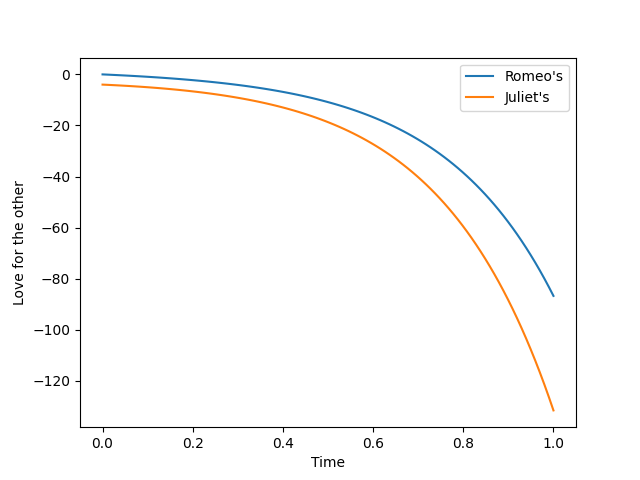
\includegraphics[width=10cm]{images/eager_beaver_1.png}
    \end{center}
    \caption{The love between two eager beaver}
\end{figure}\\
Giải thích các đoạn code trong \textit{Python} vẽ đồ thị ví dụ trên (các đoạn code này được ta định nghĩa trong file \textbf{trajectory.py} và sẽ được dùng để vẽ \textbf{phase portrait}) như sau:
\begin{itemize}
    \item Nạp các modules cần thiết, bao gồm: \textbf{numpy} (module toán học xử lý ma trận và mảng), \textbf{matplotlib.pyplot}(module đồ họa vẽ đồ thị), \textbf{math} và khai báo ma trận hệ số (hình 2).
    \begin{figure}[h!]
        \begin{center}
        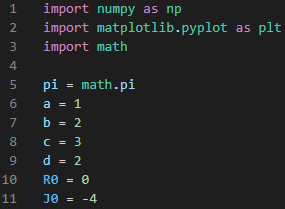
\includegraphics[width=5cm]{images/module_param.png}
        \end{center}
        \caption{Modules và khai báo}
    \end{figure}
    \item Viết hàm tính $\Delta$ và $\lambda$ (hình 3).
    \begin{figure}[h!]
        \begin{center}
        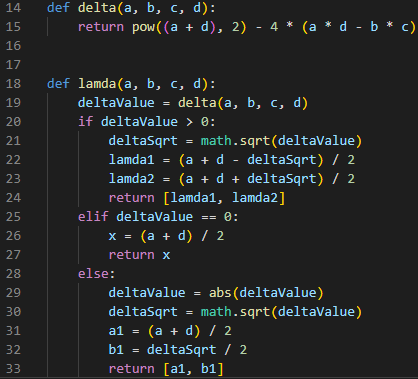
\includegraphics[width=8cm]{images/delta_lambda.png}
        \end{center}
        \caption{$\Delta$ và $\lambda$}
    \end{figure}
    \item Viết các hàm phụ tính các hằng số trong công thức tương ứng với 3 trường hợp (hình 4).
    \begin{figure}[h!]
        \begin{center}
        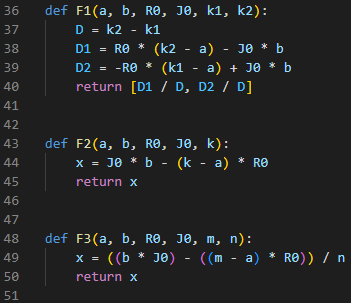
\includegraphics[width=6cm]{images/helper_func.png}
        \end{center}
        \caption{Các hàm phụ trợ tính hệ số}
    \end{figure}
    \item Hàm tính giá trị của $R$ (hình 5).
    \begin{figure}[h!]
        \begin{center}
        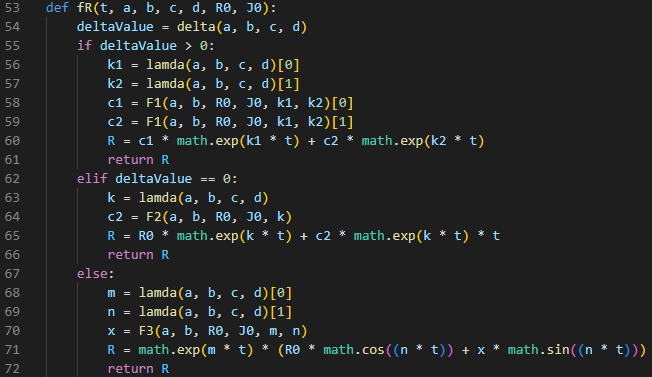
\includegraphics[width=10cm]{images/R.png}
        \end{center}
        \caption{Hàm tính giá trị $R$ theo $t$}
    \end{figure}
    \item Hàm tính giá trị của $J$ (hình 6).
    \begin{figure}[h!]
        \begin{center}
        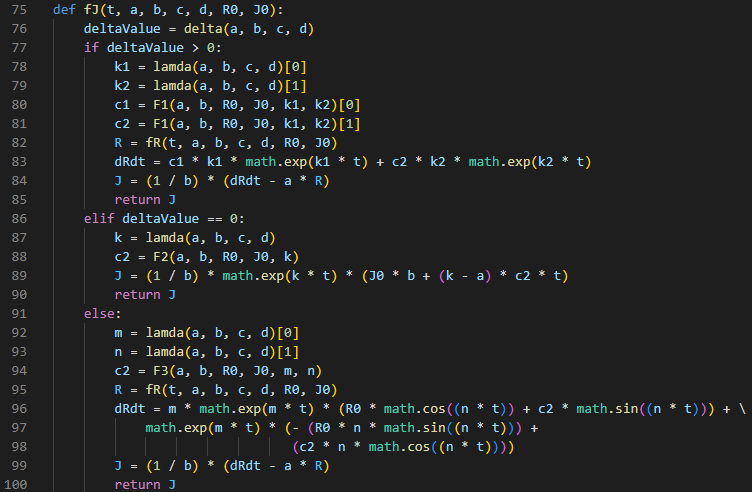
\includegraphics[width=10cm]{images/J.png}
        \end{center}
        \caption{Hàm tính giá trị $J$ theo $t$}
    \end{figure}
    \item Lấy 100 giá trị của biến thời gian $t$ trong khoảng $[0,1]$ để vẽ đồ thị (hình 7).
    \begin{figure}[h!]
        \begin{center}
        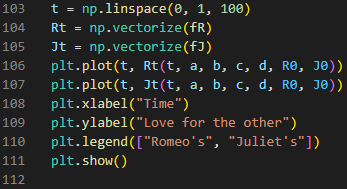
\includegraphics[width=5cm]{images/trajectory.png}
        \end{center}
        \caption{Vẽ đồ thị}
    \end{figure}
\end{itemize}
\subsubsection{Ví dụ 2}
\begin{align*}
    \begin{cases}
        R'=R+2J\\
        J'=3R+2J\\
        R(0)=1\\
        J(0)=2
    \end{cases}
\end{align*}
Tương tự ví dụ 1 nhưng $R_0=1, J_0=2$
Áp dụng công thức nghiệm chính xác ở trường hợp 1:
\begin{align*}
    \begin{cases}
        R(t)=-\frac{1}{5}e^{-t}+\frac{6}{5}e^{4t}\\
        J(t)=\frac{1}{5}e^{-t}+\frac{9}{5}e^{4t}
    \end{cases}
\end{align*}
Đồ thi biểu diễn như sau (hình 8):
\begin{figure}[h!]
    \begin{center}
    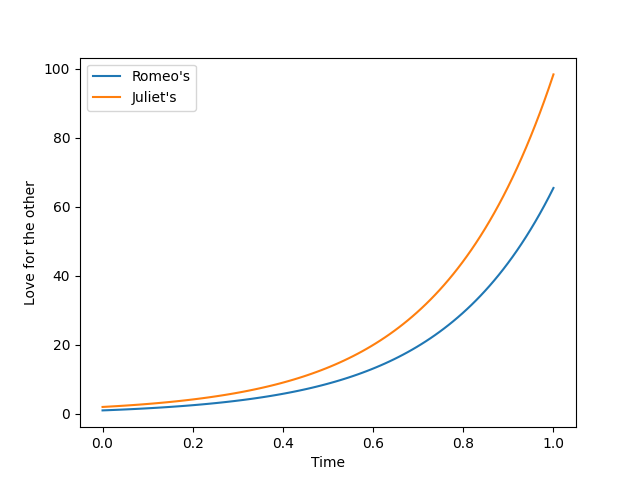
\includegraphics[width=10cm]{images/eager_beaver_2.png}
    \end{center}
    \caption{The love between two eager beaver}
\end{figure}
\subsubsection{Phase portrait}
Ứng với hệ phương trình trong 2 ví dụ trên với các điều kiện ban đầu bất kì
$\begin{cases}
        R'=R+2J\\
        J'=3R+2J
\end{cases}$
ta có phase portrait trong mặt phẳng $RJ$ được biểu diễn trong hình 9
\begin{figure}[h!]
    \begin{center}
    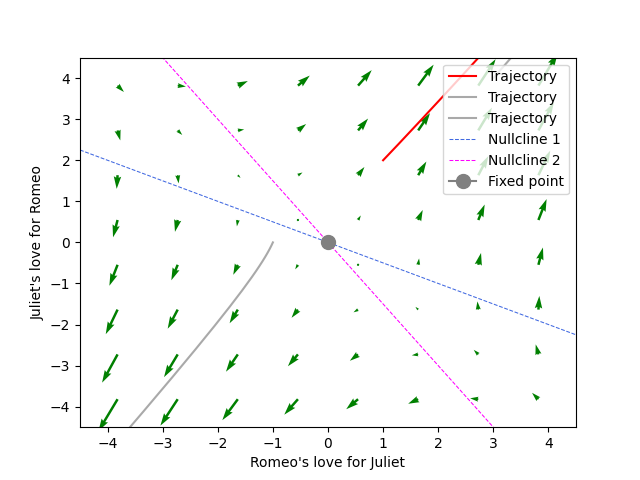
\includegraphics[width=10cm]{images/phase_portrait_eager_beaver.png}
    \end{center}
    \caption{The phase portrait of the love between two eager beaver}
\end{figure}\\
Giải thích các đoạn code trong \textit{Python} vẽ phase portrait:
\begin{itemize}
    \item Nạp các modules cần thiết, bao gồm \textbf{numpy}, \textbf{matplotlib.pyplot}, package \textbf{odeint} trong module \textbf{scipy.integrate} (dùng để giải hệ phương trình vi phân), các thông số $a, b, c, d, R_0, J_0$ trong module \textbf{trajectory} (module này đã được ta định nghĩa). Ta sẽ vẽ các trajectory ứng với các bộ giá trị ban đầu $[R_0, J_0], [R_0+2,J_0+2], [R_0-2,J_0-2]$ (hình 10).
    \begin{figure}[h!]
        \begin{center}
        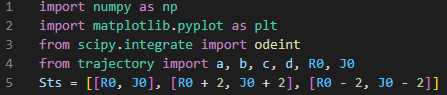
\includegraphics[width=8cm]{images/pakage_init.png}
        \end{center}
        \caption{Modules, pakage và khai báo các bộ giá trị ban đầu}
    \end{figure}
    \item Viết hàm biểu diễn hệ phương trình vi phân (hình 11).
    \begin{figure}[h!]
        \begin{center}
        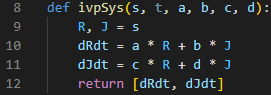
\includegraphics[width=5cm]{images/ivpSys.png}
        \end{center}
        \caption{Hàm biểu diễn hệ phương trình vi phân}
    \end{figure}
    \item Vẽ các vector biểu diễn $R'$ và $J'$ tại thời điểm ban đầu $t=0$ của một tập gồm 144 điểm rời rạc $(R_0,J_0)$ phân bố đều nhau trên mặt phẳng $RJ$ (hình 12).
    \begin{figure}[h!]
        \begin{center}
        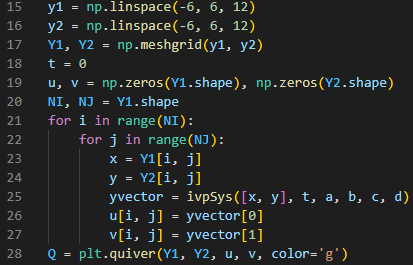
\includegraphics[width=8cm]{images/vector_field.png}
        \end{center}
        \caption{Vẽ các vector biểu diễn $R'$ và $J'$}
    \end{figure}
    \item Vẽ các trajectory với 200 giá trị của biến thời gian $t$ từ $(0, 5)$ ứng với 3 bộ giá trị ban đầu: $(R_0, J_0)$ (màu đỏ) và $(R_0 + 2, J_0 + 2), (R_0 - 2, J_0 - 2)$ (màu xám) (hình 13).
    \begin{figure}[h!]
        \begin{center}
        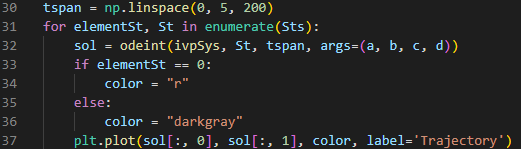
\includegraphics[width=10cm]{images/plot_odeint.png}
        \end{center}
        \caption{Vẽ các trajectory}
    \end{figure}
    \item Ký hiệu các chú thích và vẽ phase portrait (hình 14).
    \begin{figure}[h!]
        \begin{center}
        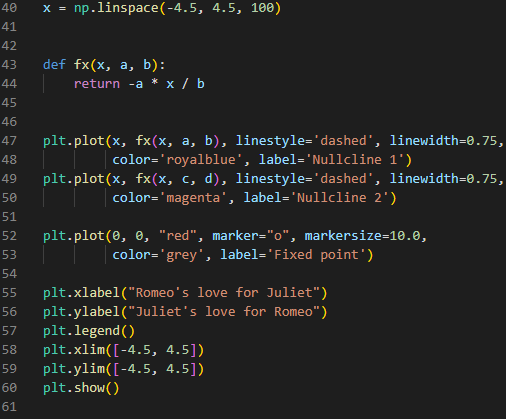
\includegraphics[width=10cm]{images/phase_portrait.png}
        \end{center}
        \caption{Vẽ phase portrait}
    \end{figure}
\end{itemize}
\subsection{Narcissistic Nerd}
Điều kiện của a, b trong phong cách này là $a > 0$ và $b < 0$. Ta xét 2 ví dụ cùng ma trận hệ số nhưng điều kiện ban đầu khác nhau. Đoạn code trong \textit{Python} dùng để vẽ các đồ thị và phase portrait tương tự mục Eager Beaver, chỉ thay đổi tham số $a, b, c, d, R_0, J_0$.
\subsubsection{Ví dụ 1}
\begin{align*}
    \begin{cases}
        R'=5R-J\\
        J'=R+3J\\
        R(0)=1\\
        J(0)=2
    \end{cases}
\end{align*}
Theo bài 1, ta có $\Delta=0$, hệ có 1 trị riêng duy nhất $\lambda=4$. Áp dụng công thức nghiệm chính xác ở trường hợp 3:
\begin{align*}
    \begin{cases}
        R(t)=e^{4t}(-t+1)\\
        J(t)=e^{4t}(-t+2)
    \end{cases}
\end{align*}
Biểu diễn $R$ (narcissistic nerd) và $J$ (eager beaver) trên cùng một đồ thị theo biến thời gian $t$ (hình 15):
\begin{figure}[h!]
    \begin{center}
    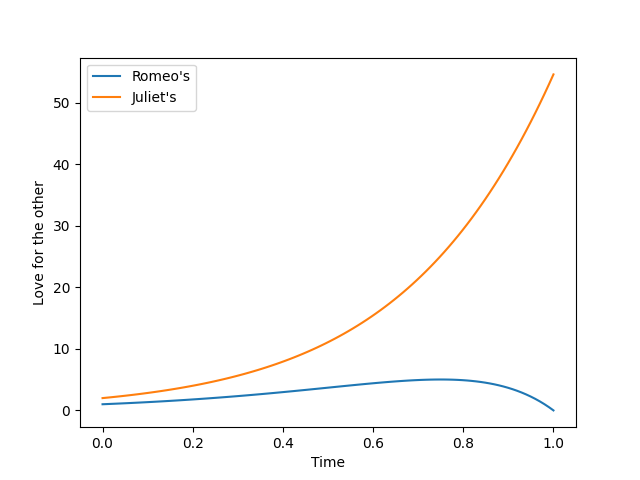
\includegraphics[width=10cm]{images/narcissistic_nerd_1.png}
    \end{center}
    \caption{The love between a narcissistic nerd and a eager beaver}
\end{figure}
\subsubsection{Ví dụ 2}
\begin{align*}
    \begin{cases}
        R'=5R-J\\
        J'=R+3J\\
        R(0)=1\\
        J(0)=3
    \end{cases}
\end{align*}
Tương tự ví dụ 1 nhưng $R_0 = 1, J_0 = 3$ Áp dụng công thức nghiệm chính xác ở trường hợp 3:
\begin{align*}
    \begin{cases}
        R(t)=e^{4t}(-2t+1)\\
        J(t)=e^{4t}(-2t+3)
    \end{cases}
\end{align*}
Đồ thị biểu diễn ở hình 16.
\begin{figure}[h!]
    \begin{center}
    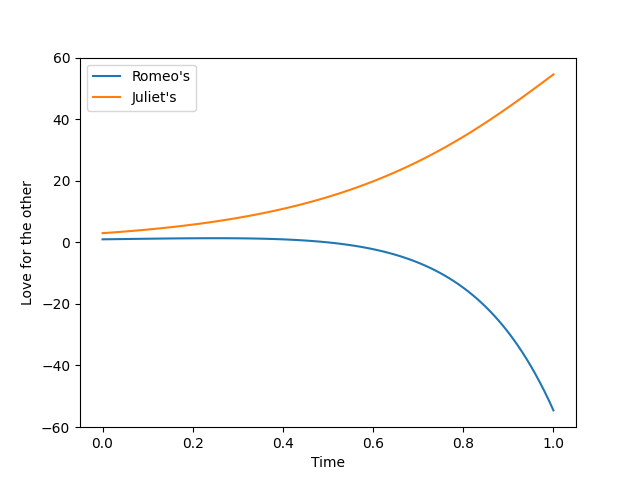
\includegraphics[width=10cm]{images/narcissistic_nerd_2.png}
    \end{center}
    \caption{The love between a narcissistic nerd and a eager beaver}
\end{figure}
\subsubsection{Phase portrait}
Ứng với hệ phương trình trong 2 ví dụ trên với các điều kiện ban đầu bất kì
$\begin{cases}
        R'=5R-J\\
        J'=R+3J
\end{cases}$
ta có phase portrait trong mặt phẳng $RJ$ được biểu diễn trong hình 17.
\begin{figure}[h!]
    \begin{center}
    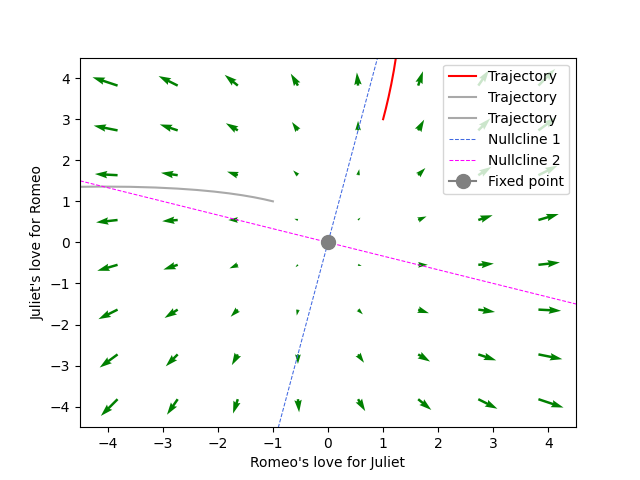
\includegraphics[width=10cm]{images/phase_portrait_narcissistic_nerd.png}
    \end{center}
    \caption{The phase portrait of the love between a narcissistic nerd and a eager beaver}
\end{figure}
\subsection{Cautious Lover}
Điều kiện của a, b trong phong cách này là $a < 0$ và $b > 0$. Ta xét 2 ví dụ cùng ma trận hệ số nhưng điều kiện ban đầu khác nhau. Đoạn code trong \textit{Python} dùng để vẽ các đồ thị và phase portrait tương tự mục Eager Beaver, chỉ thay đổi tham số $a, b, c, d, R_0, J_0$.
\subsubsection{Ví dụ 1}
\begin{align*}
    \begin{cases}
        R'=-3R+9J\\
        J'=-2R+3J\\
        R(0)=1\\
        J(0)=2
    \end{cases}
\end{align*}
Theo bài 1, ta có $\Delta=-36<0$, hệ có 2 trị riêng phức liên hợp $\lambda_{1,2}= \pm 3i$. Áp dụng công thức nghiệm chính xác ở trường hợp 2:
\begin{align*}
    \begin{cases}
        R(t)=\cos{3t}+5\sin{3t}\\
        J(t)=2\cos{3t}+\frac{4}{3}\sin{3t}
    \end{cases}
\end{align*}
Biểu diễn $R$ (cautious lover) và $J$ (narcissistic nerd) trên cùng một đồ thị theo biến thời gian $t$ (hình 18):
\begin{figure}[h!]
    \begin{center}
    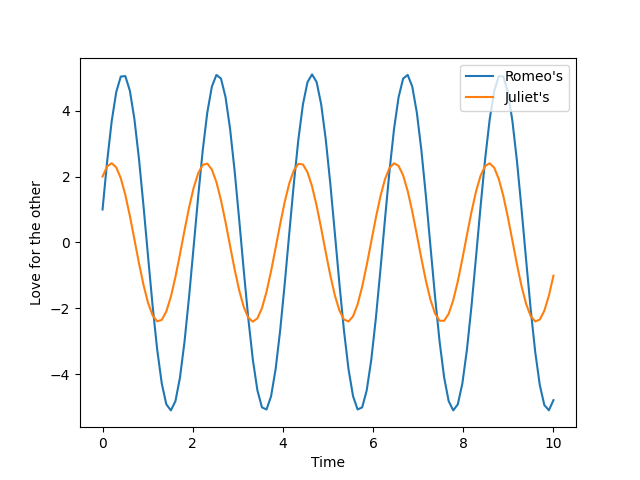
\includegraphics[width=10cm]{images/cautious_lover_1.png}
    \end{center}
    \caption{The love between a cautious lover and a narcissistic nerd}
\end{figure}
\subsubsection{Ví dụ 2}
\begin{align*}
    \begin{cases}
        R'=-3R+9J\\
        J'=-2R+3J\\
        R(0)=2\\
        J(0)=-4
    \end{cases}
\end{align*}
Tương tự ví dụ 1 nhưng $R_0 = 2, J_0 = -4$ Áp dụng công thức nghiệm chính xác ở trường hợp 2:
\begin{align*}
    \begin{cases}
        R(t)=2\cos{3t}-14\sin{3t}\\
        J(t)=-4\cos{3t}-\frac{16}{3}\sin{3t}
    \end{cases}
\end{align*}
Đồ thị biểu diễn ở hình 19.
\begin{figure}[h!]
    \begin{center}
    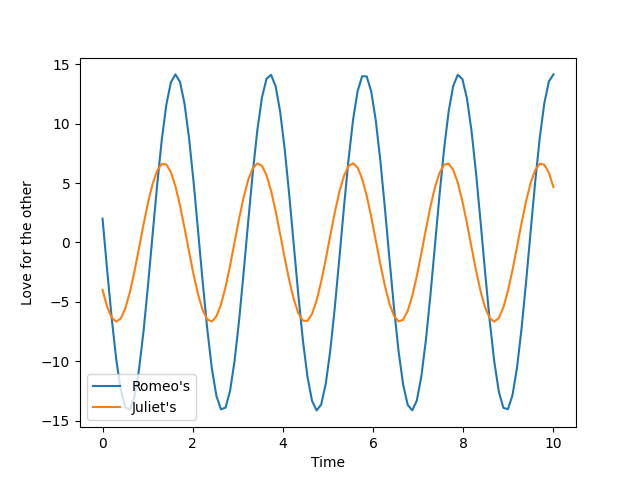
\includegraphics[width=10cm]{images/cautious_lover_2.png}
    \end{center}
    \caption{The love between a cautious lover and a narcissistic nerd}
\end{figure}
\subsubsection{Phase portrait}
Ứng với hệ phương trình trong 2 ví dụ trên với các điều kiện ban đầu bất kì
$\begin{cases}
        R'=-3R+9J\\
        J'=-2R+3J
\end{cases}$
ta có phase portrait trong mặt phẳng $RJ$ được biểu diễn trong hình 20.
\begin{figure}[h!]
    \begin{center}
    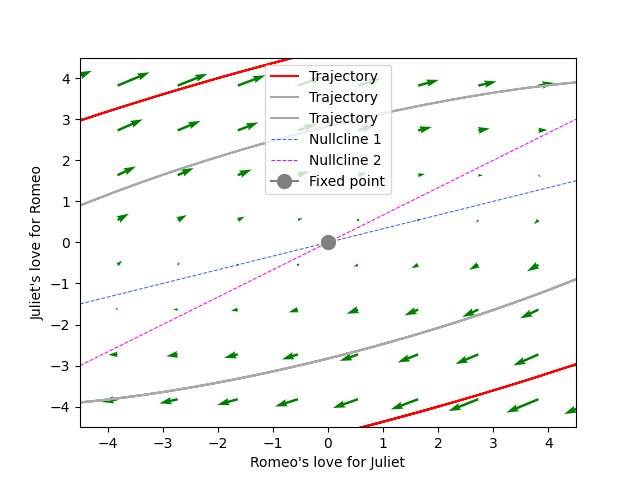
\includegraphics[width=10cm]{images/phase_portrait_cautious_lover.png}
    \end{center}
    \caption{The phase portrait of the love between a cautious lover and a narcissistic nerd}
\end{figure}
\subsection{Hermit}
Điều kiện của a, b trong phong cách này là $a < 0$ và $b < 0$. Ta xét 2 ví dụ cùng ma trận hệ số nhưng điều kiện ban đầu khác nhau. Đoạn code trong \textit{Python} dùng để vẽ các đồ thị và phase portrait tương tự mục Eager Beaver, chỉ thay đổi tham số $a, b, c, d, R_0, J_0$.
\subsubsection{Ví dụ 1}
\begin{align*}
    \begin{cases}
        R'=-3R-13J\\
        J'=5R-J\\
        R(0)=3\\
        J(0)=1
    \end{cases}
\end{align*}
Theo bài 1, ta có $\Delta=-256<0$, hệ có 2 trị riêng phức liên hợp $\lambda_{1,2}=-2\pm8i$. Áp dụng công thức nghiệm chính xác ở trường hợp 2:
\begin{align*}
    \begin{cases}
        R(t)=e^{-2t}(3\cos{8t}-2\sin{8t})\\
        J(t)=e^{-2t}(\cos{8t}+2\sin{8t})
    \end{cases}
\end{align*}
Biểu diễn $R$ (hermit) và $J$ (cautious lover) trên cùng một đồ thị theo biến thời gian $t$ (hình 21):
\begin{figure}[h!]
    \begin{center}
    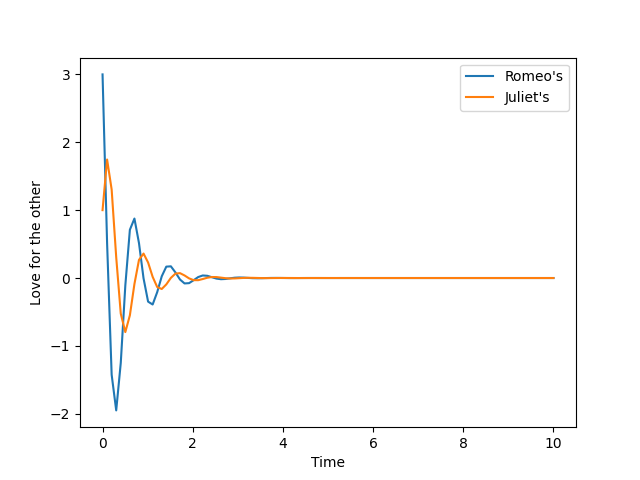
\includegraphics[width=10cm]{images/hermit_1.png}
    \end{center}
    \caption{The love between a hermit and a cautious lover}
\end{figure}
\subsubsection{Ví dụ 2}
\begin{align*}
    \begin{cases}
        R'=-3R-13J\\
        J'=5R-J\\
        R(0)=2\\
        J(0)=-2
    \end{cases}
\end{align*}
Tương tự ví dụ 1 nhưng $R_0 = 2, J_0 = -2$ Áp dụng công thức nghiệm chính xác ở trường hợp 2:
\begin{align*}
    \begin{cases}
        R(t)=e^{-2t}(2\cos{8t}+3\sin{8t})\\
        J(t)=e^{-2t}(-2\cos{8t}+\sin{8t})
    \end{cases}
\end{align*}
Đồ thị biểu diễn ở hình 22.
\begin{figure}[h!]
    \begin{center}
    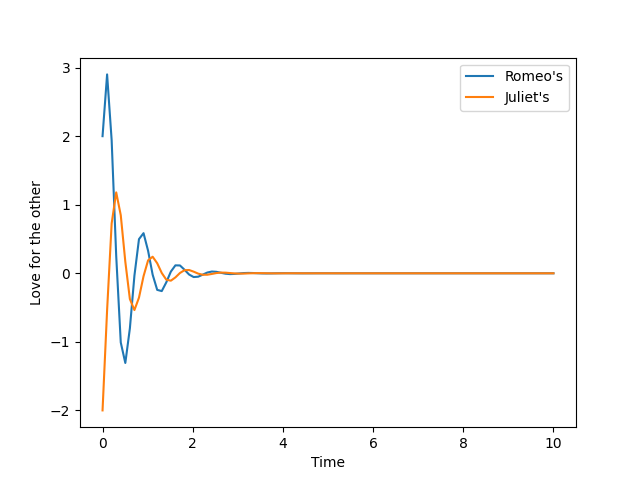
\includegraphics[width=8cm]{images/hermit_2.png}
    \end{center}
    \caption{The love between a hermit and a cautious lover}
\end{figure}
\subsubsection{Phase portrait}
Ứng với hệ phương trình trong 2 ví dụ trên với các điều kiện ban đầu bất kì
$\begin{cases}
        R'=-3R-13J\\
        J'=5R-J
\end{cases}$
ta có phase portrait trong mặt phẳng $RJ$ được biểu diễn trong hình 23.
\begin{figure}[h!]
    \begin{center}
    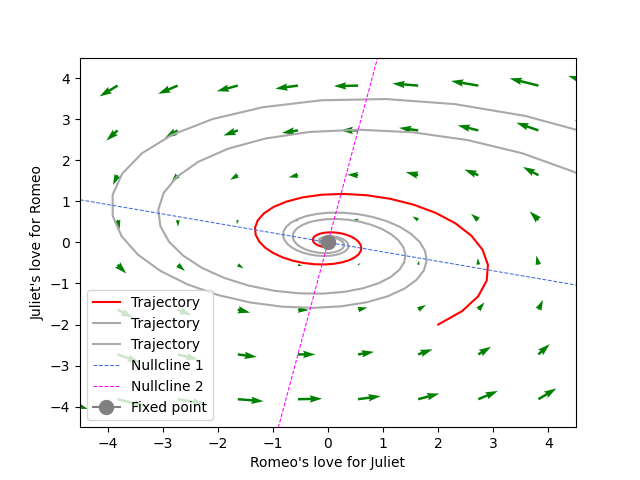
\includegraphics[width=9cm]{images/phase_portrait_hermit.png}
    \end{center}
    \caption{The phase portrait of the love between a hermit and a cautious lover}
\end{figure}